\documentclass[12pt]{ucthesis}

\usepackage{etex}
\usepackage[morefloats=125]{morefloats}
\usepackage[hyphens]{url}
\usepackage[caption=false]{subfig}
\usepackage{graphicx}
\usepackage{tabularx}
\usepackage{amssymb}
\usepackage{amsmath}
\usepackage{amsthm}
\usepackage{enumitem} 
\usepackage[letterpaper]{geometry}
\usepackage[overload]{textcase}
\usepackage{color}
\usepackage[nonumberlist,toc]{glossaries}
\usepackage{wrapfig}
\usepackage{longtable}
\usepackage{morefloats}
\usepackage{float}
\usepackage{listings}
\usepackage{makecell}
\usepackage{appendix}
\usepackage[]{algorithm2e}
\usepackage{titlesec}
\usepackage[breaklinks=true,hidelinks,pdfusetitle]{hyperref}
\usepackage{cleveref}
\usepackage{ifthen}

\setcounter{secnumdepth}{3}
\setcounter{tocdepth}{3}

% Add definitions, etc.

\newtheorem{theorem}{Theorem}
\newtheorem{proposition}{Proposition}

\theoremstyle{definition}
\newtheorem{definition}{Definition}

\newtheorem{example}[definition]{Example}

\theoremstyle{remark}
\newtheorem*{remark}{Remark}

\newcommand{\dif}{\mathrm{d}} % For the differential operator, d

% Added to avoid windows and orphans
\usepackage[all]{nowidow}
% Added to fix spacing between footnote entries
\usepackage{setspace}
\newlength{\myfootnotesep}
\setlength{\myfootnotesep}{\baselineskip}
\addtolength{\myfootnotesep}{-\footnotesep}
\setlength{\footnotesep}{\myfootnotesep} % set spacing between footnotes

\makeindex
\makeglossaries

% Shrink the size of headers
\titleformat{\chapter}[display]
        {\normalfont\normalsize\centering}
        {\ifthenelse{\equal{\thechapter}{A}}{APPENDICES\\[4.3ex]}{}\chaptertitlename\ \thechapter}
        {0pt}{\normalsize\uppercase}
\titlespacing*{\chapter}{0pt}{-20pt}{4.3ex plus .2ex}


\titleformat*{\section}{\normalsize\bfseries}
\titleformat*{\subsection}{\small\bfseries}
\titleformat*{\subsubsection}{\small\bfseries}
\titleformat*{\paragraph}{\small\bfseries}
\titleformat*{\subparagraph}{\small\bfseries}

\bibliographystyle{abbrv}

% Make \tindent indent pages if you have no paragraph indent
\newlength\tindent
\setlength{\tindent}{\parindent}
\setlength{\parindent}{0.in} \setlength{\parskip}{1.em}
\renewcommand{\indent}{\hspace*{\tindent}}
% Otherwise, comment out the above and uncomment this for default indentation on each paragraph
%\setlength{\parindent}{0.25in} \setlength{\parskip}{6pt}

\geometry{verbose,nohead,tmargin=1in,bmargin=1in,lmargin=1.5in,rmargin=1in}

% Different font in captions (single-spaced, bold) ------------
\newcommand{\captionfonts}{\small\bf\ssp}

\newcommand{\mycaption}[2]{\caption[#1 --- #2]{#1 --- #2}}

\makeatletter  % Allow the use of @ in command names
\long\def\@makecaption#1#2{%
  \vskip\abovecaptionskip
  \sbox\@tempboxa{{\captionfonts #1: #2}}%
  \ifdim \wd\@tempboxa >\hsize
    {\captionfonts #1: #2\par}
  \else
    \hbox to\hsize{\hfil\box\@tempboxa\hfil}%
  \fi
  \vskip\belowcaptionskip}
\makeatother   % Cancel the effect of \makeatletter
% ---------------------------------------

% Define Appendix refs
\crefname{app}{appendix}{appendices}
\Crefname{app}{Appendix}{Appendices}

% Add Figures folder to the graphics path
\graphicspath{{Figures/}{figures/}}

% Options for hyperref
\hypersetup{
    bookmarksnumbered=true,
    bookmarksopen=false,
    bookmarksopenlevel=0,
    colorlinks=false,
    pdfstartview=Fit,
    pdfborder={0 0 0},
}

\newcounter{qcounter}
\providecommand{\keywords}[1]{\textbf{\textit{Keywords:}} #1}


\begin{document}

% Declarations for Front Matter
\title{Representation Theory in Physical Groups}
\author{Jaxon Green}
\degreeyear{August} \degreeyear{2024} \degree{Master of Science}
\defensemonth{August} 
\defenseyear{2024}
\numberofmembers{3}
   \chair{Sean Gasiorek \linebreak Professor of Mathematics}
   \othermemberA{Elena Dimitrova\linebreak Professor of Mathematics}
   \othermemberB{Robert Easton\linebreak Professor of Mathematics}
\field{Mathematics} \campus{San Luis Obispo}
\copyrightyears{seven}


\maketitle

\begin{frontmatter}

% Custom made for Cal Poly (by Mark Barry, modified by Andrew Tsui).
\copyrightpage

% Custom made for Cal Poly (by Andrew Tsui).
\committeemembershippage

\begin{abstract}
A representation is a group homomorphism whose image is a group of invertible matrices. Representations and their associated matrices are analyzed through well-established techniques from linear algebra. We characterize representations by a unique decomposition into irreducible representations just as we characterize the decomposition of matrices into their eigenspaces. Through the study of these representations, we uncover mathematical relationships that underlie groups with physical applications. Due to physical symmetries, we study how the irreducible representations of groups that embody the actions of even the most basic rotations are utilized in the computation of irreducible representations groups that reflect more complicated mechanics, like the Poincar\'e Group. Further, we utilize the representations of the abstract braid group to gain key insights into understanding the behavior of anyonic systems in quantum mechanics. Finally, we explore the behavior of Fibonacci anyons for ways to understand to illustrate the underlying braid relations.
\end{abstract}

\begin{acknowledgements}
I would like to thank my dog Fluffy and Darth Vader. 
\end{acknowledgements}

\tableofcontents

%\listoftables

\listoffigures

% Add CHAPTER into table of contents.
\addtocontents{toc}{%
   \noindent CHAPTER
}

\end{frontmatter}

\pagestyle{plain}

\renewcommand{\baselinestretch}{1.66}

\chapter{Introduction}

A representation is a group homomorphism whose image is a group of invertible matrices. At a glance, representations give us the ability to dial back the complexity of a mysterious group by viewing its elements as matrices. Thanks to the rigorous development of linear algebra, groups of matrices are well-understood structures. Representations allow us to unravel the mystery of any unknown group's structure and reveal a group’s fundamental properties as the result of linear algebra techniques. This is especially useful to us when a group is constructed to reflect the behavior of physical phenomena. In this thesis, the groups we will study create rigorous definitions for physical actions such as rotations, translations, relativistic transformations, and interactions of particles in quantum systems. In the search for representations of these groups, we utilize physical symmetries observed in the real world to make generalizable calculations. That is, we can use representations of groups that reflect simple physical actions to generate representations of the groups corresponding to more complicated physical actions. The primary objective in our study of representation theory is to seek a method to characterize properties of physical systems as the direct result of properties of the mathematical structures that underlie them.

Representation theory is already a well-documented and researched subject. In fact, the study of representation theory may be approached through the lens of many different fields in mathematics. To name a few, combinatorics, category theory, and abstract algebra all play a hand in the rigorous development of this subject. In this thesis, we sample many of these disciplines, finding connections between these seemingly disparate fields of study, to gain deeper insight into the structure of representations. For sake of time, this sampling of each discipline is nowhere near a complete examination of every facet of representation theory. Instead, the main work done in this thesis seeks to create a streamlined approach to studying representations while pointing out necessary developments from other branches of mathematics to make our examination rigorous. To this end, many of the theorems and concepts that different sources regard as accepted truth in their studies are explicitly proved here. It is the hope that readers should find the study of representation theory accessible even if they do not have expertise in the more niche fields of mathematics.

\chapter{Classical Algebraic Geometry} \label{classical}

First Chapter stuff

\section{First Section Title}

And now the math begins\dots

\begin{definition}
Given a collection of polynomials $I\subseteq k[x_{1},..., x_{n}]$, the \textbf{affine variety} determined by $I$ is the set
\[
\mathbf{V}(I)=\left\{\mathbf{a}\in k^n\,|\,f(\mathbf{a})=0\text{ for all }f\in I\right\}\subseteq k^n.
\]
This set is sometimes also called the {\bfseries vanishing locus} or {\bfseries zero locus} of $I$. If $I=\lbrace f_{1},..., f_{n}\rbrace$ is a finite collection of polynomials, we we write simply $\mathbf{V}(f_{1},..., f_{n})$.
\end{definition}

\begin{example}
The standard real plane parabola is the affine variety $\mathbf{V}(y-x^{2})$ in ${\bf R}^2$:
\begin{figure}[ht]
    \centering
    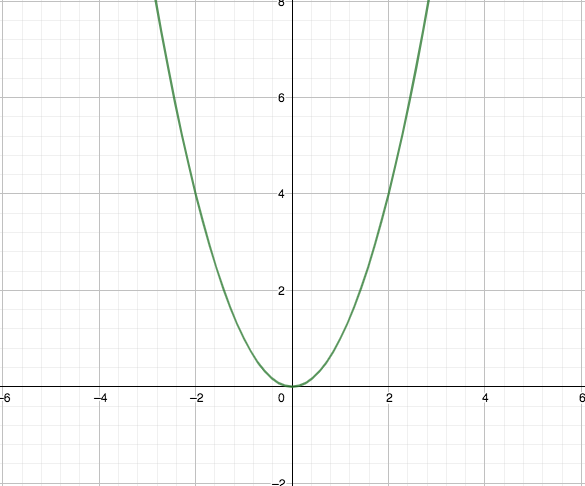
\includegraphics[scale=.25]{Parabolavariety.png}
    %\caption{$y-x^{2}=0$}
\end{figure}
\end{example}


\subsection{Relevant subsection title}


\chapter{A New Hope}

\section{Relevant section title}

\subsection{Also relevant}

\subsubsection{Maybe too many subsections}

\nocite{*}
\bibliography{bibliography}

% Indents Appendix in Table of Contents
\makeatletter
\addtocontents{toc}{\let\protect\l@chapter\protect\l@section}
\makeatother

% Hack to make Appendices to appear in Table of Contents
\addtocontents{toc}{%
   \noindent APPENDICES
}
\begin{appendices}


\end{appendices}

\end{document}
